% rua-harness paper. Target: ICML 2027.
% Style files are the ICML 2026 kit (2027 not published yet). See README.md.
\documentclass{article}

\usepackage{microtype}
\usepackage{graphicx}
\usepackage{subcaption}
\usepackage{booktabs}
\usepackage{adjustbox}  % generated tables shrink to fit
\usepackage{hyperref}
\newcommand{\theHalgorithm}{\arabic{algorithm}}

% Blind review version. Use [preprint] or [accepted] later.
\usepackage{icml2026}

\usepackage{amsmath}
\usepackage{amssymb}
\usepackage{mathtools}
\usepackage{xcolor}
\usepackage{tikz}
\usetikzlibrary{positioning,arrows.meta,shapes.geometric,fit,backgrounds}
\usepackage[capitalize,noabbrev]{cleveref}
\usepackage[textsize=tiny]{todonotes}

\newcommand{\dem}{DEM}
\newcommand{\draftnote}[1]{\textcolor{red}{[#1]}}

\icmltitlerunning{Command Formats for Agent to Policy Handoff}

\begin{document}

\twocolumn[
  \icmltitle{What Should an Agent Tell a Robot Policy?\\
    Command Formats for Handing Physical Jobs to a Small Fast Policy}

  \icmlsetsymbol{equal}{*}
  \begin{icmlauthorlist}
    \icmlauthor{Adi Kothari}{yale}  % confirm full names before submission
    \icmlauthor{William Gu}{yale}
    \icmlauthor{Xiatao Sun}{yale}
  \end{icmlauthorlist}
  \icmlaffiliation{yale}{APOLLO Lab, Yale University, New Haven, CT, USA}
  \icmlcorrespondingauthor{Adi Kothari}{TBD}
  \icmlkeywords{Robot learning, LLM agents, imitation learning, RoboCasa}
  \vskip 0.3in
]

\printAffiliationsAndNotice{}

% DRAFT abstract for the Jan 14 deadline (Part T, 2026-11-27). About 150
% words. Every bold bracket is a placeholder; no number in it is real yet.
\begin{abstract}
\draftnote{DRAFT: placeholders in brackets; no result is real yet.}
LLM agents can plan household jobs, but driving a robot step by step makes
them slow and costly in tokens. A small learned policy acts fast, but must be
told what to do. We ask what form that command should take. We compare five
formats: a sentence, structured text, 2D points drawn on the camera images,
3D points given as extra input tokens, and a path of future gripper poses.
For each format we retrain the same policy, DEM, on the same RoboCasa
demonstrations, labeling points in hindsight from where the gripper closed
and opened. On 18 kitchen tasks, \textbf{[best format]} reaches
\textbf{[X\%]} success with perfect commands against \textbf{[Y\%]} for a
sentence, and \textbf{[Z\%]} on held-out objects. With commands written by
an LLM agent, it reaches \textbf{[A\%]}. Paired with the agent, the policy
matches the agent alone within \textbf{[B]} points while using
\textbf{[C$\times$]} fewer tokens and \textbf{[D$\times$]} less time. We
release code, labels and per-episode results.
\end{abstract}

\section{Introduction}
\label{sec:intro}

\draftnote{DRAFT stub.}

\begin{figure*}[t]
  \centering
  \resizebox{\textwidth}{!}{% Figure 1 draft: request -> LLM agent -> command -> policy -> simulator.
% Needs tikz with libraries positioning, arrows.meta (loaded in main.tex).
% Example command follows ATOMIC_SEEN["PickPlaceCounterToCabinet"] in rua_harness/command.py.
% Pixel values are illustrative, not from a real episode.
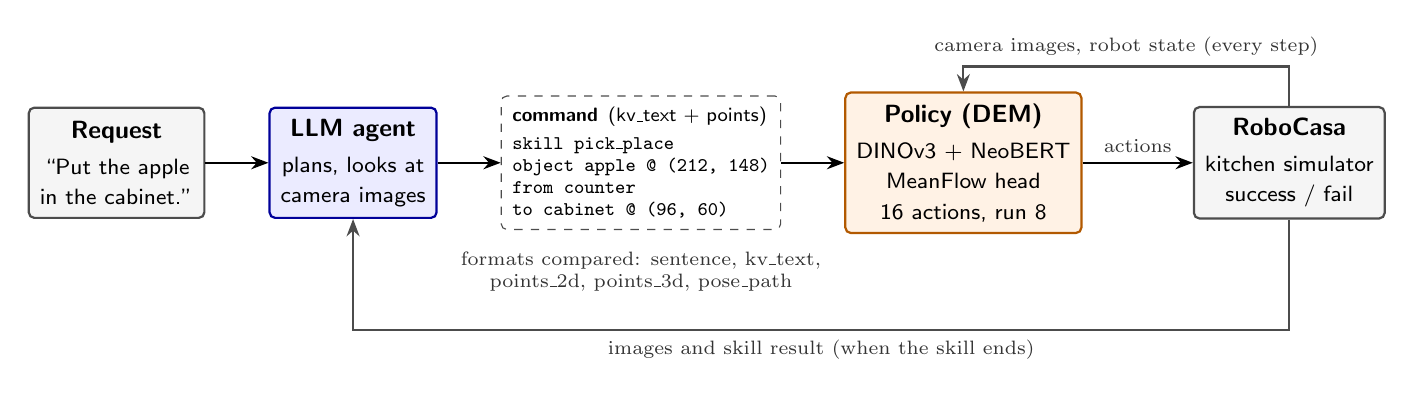
\begin{tikzpicture}[
    font=\sffamily\small,
    node distance=5mm and 8mm,
    box/.style={draw, rounded corners=2pt, thick, align=center, minimum height=14mm, inner sep=4pt},
    agent/.style={box, fill=blue!8, draw=blue!60!black},
    policy/.style={box, fill=orange!10, draw=orange!70!black},
    io/.style={box, fill=gray!8, draw=gray!60!black},
    cmd/.style={draw=gray!60!black, dashed, rounded corners=2pt, fill=white, align=left, inner sep=4pt, font=\ttfamily\scriptsize},
    arr/.style={-{Stealth[length=2.2mm]}, thick},
    lab/.style={font=\scriptsize, text=gray!40!black},
  ]
  \node[io] (req) {\textbf{Request}\\[2pt]\footnotesize ``Put the apple\\\footnotesize in the cabinet.''};
  \node[agent, right=of req] (agent) {\textbf{LLM agent}\\[2pt]\footnotesize plans, looks at\\\footnotesize camera images};
  \node[cmd, right=of agent] (cmd) {%
    {\sffamily\bfseries command} {\sffamily(kv\_text + points)}\\[2pt]
    skill  pick\_place\\
    object apple   @ (212, 148)\\
    from   counter\\
    to     cabinet @ (96, 60)};
  \node[policy, right=of cmd] (policy) {\textbf{Policy (DEM)}\\[2pt]\footnotesize DINOv3 + NeoBERT\\\footnotesize MeanFlow head\\\footnotesize 16 actions, run 8};
  \node[io, right=14mm of policy] (sim) {\textbf{RoboCasa}\\[2pt]\footnotesize kitchen simulator\\\footnotesize success / fail};

  \draw[arr] (req) -- (agent);
  \draw[arr] (agent) -- (cmd);
  \draw[arr] (cmd) -- (policy);
  \draw[arr] (policy) -- node[lab, above]{actions} (sim);
  % feedback: images and state to the policy every step, result to the agent at the end
  \draw[arr, gray!60!black] (sim.north) -- ++(0,5mm) -| node[lab, pos=0.25, above]{camera images, robot state (every step)} (policy.north);
  \draw[arr, gray!60!black] (sim.south) -- ++(0,-14mm) -| node[lab, pos=0.25, below]{images and skill result (when the skill ends)} (agent.south);

  \node[lab, below=1.5mm of cmd, align=center] {formats compared: sentence, kv\_text,\\points\_2d, points\_3d, pose\_path};
\end{tikzpicture}
}
  \caption{\draftnote{Draft.} A request goes to the LLM agent. The agent
  writes a short command, here in structured form with points. The policy
  turns the command and camera images into actions in the simulator. We vary
  the command format and retrain the policy for each.}
  \label{fig:overview}
\end{figure*}

Points to make:
\begin{itemize}
  \item LLM agents plan well but act slowly and cost tokens when they drive a robot step by step.
  \item Small policies act fast but need a command. The format of that command is a design choice nobody has measured with the policy retrained per format.
  \item We measure it: five formats, same policy architecture, same data, RoboCasa atomic tasks.
  \item Contributions: (1) a controlled comparison of command formats; (2) agent alone vs.\ agent plus policy on success, time and tokens; (3) open code and per-episode CSVs.
\end{itemize}

\section{Related Work}
\label{sec:related}

\draftnote{DRAFT stub. Fill citations in refs.bib.}

\paragraph{LLM agents for robots.} Agents that call skills or write code
(SayCan, Code as Policies, HexaShell). \draftnote{cite}

\paragraph{Language-conditioned policies.} Vision-language-action models and
small policies conditioned on text. \draftnote{cite}

\paragraph{Points, traces and poses as commands.} Policies conditioned on 2D
points, sketched traces or goal poses. \draftnote{cite}

\paragraph{Benchmarks.} RoboCasa and its target split. \draftnote{cite}

\section{Method}
\label{sec:method}

% DRAFT (Part T, 2026-11-27). Written from the code on branch overnight-nov26:
% rua_harness/command.py, policy/{model,variants,data,label_commands,
% commands_gt,run_skill,train}.py, policy/commander/. Every design choice that
% has no result yet is marked with \draftnote{no result yet}.

\draftnote{DRAFT. Describes what is built. No trained-policy result exists yet.}

An LLM agent decides what to do. A small learned policy decides how to move.
Between them sits one \emph{command}: the message the agent sends each time it
hands the policy a job. We fix the command's content and vary only its
\emph{format}, the way that content is shown to the policy. For each format we
retrain the same policy on the same demonstrations.

\subsection{The command}
\label{sec:command}

A command names a skill and the things it acts on. The skills are
\texttt{pick\_place}, \texttt{open}, \texttt{close}, \texttt{slide},
\texttt{press}, \texttt{turn}, \texttt{insert} and \texttt{navigate}. Each
skill has required fields (for example, \texttt{pick\_place} needs an
\texttt{object} and a \texttt{target}) and optional ones (a \texttt{source}
name, or a \texttt{direction} such as \texttt{on} or \texttt{out}). The
\texttt{object} and \texttt{target} are references: a short name and,
optionally, a 3D point in the robot base frame where the gripper should act.

The command carries two kinds of content, and we keep them apart on purpose.
The \emph{semantic channel} is the names: skill, object, source, target,
direction. It is text and goes to the policy's frozen language encoder. The
\emph{geometric channel} is the points (or, in one format, a pose path). It
goes to a small learned encoder, or is drawn on the images. Numbers never pass
through the language encoder, and names never pass through the point encoder.

\subsection{Five command formats}
\label{sec:formats}

All formats share the same demonstrations, cameras (left and right agent
views), state, action chunk and training budget. They differ only in how the
command enters the policy.

\paragraph{\texttt{sentence}.} The original RoboCasa instruction, for example
``Open the left drawer.'' This is stock \dem{} and the control for every
other format.

\paragraph{\texttt{kv\_text}.} Structured text with a fixed field order, no
punctuation and no numbers, for example
\texttt{skill pick place object apple from counter to cabinet}. It carries the
same names as the sentence in a regular form that an agent can fill in
without writing prose. The formats below all keep this text and add geometry
to it, so each is compared against \texttt{kv\_text} as well as against
\texttt{sentence}.

\paragraph{\texttt{points\_2d}.} The grasp point and the place point are
projected into each agent-view camera and drawn on its image as filled
circles (radius 4 pixels at $256\times256$, green for grasp, red for place,
each with a dark outline). Points behind the camera or outside the image are
not drawn. The policy architecture is unchanged; it reads the points from the
pixels.

\paragraph{\texttt{points\_3d} and \texttt{points\_3d\_rgb}.} The two 3D
points, in the robot base frame of the current frame, become two extra tokens.
Each point goes through random Fourier features (16 frequencies, scale 10,
concatenated with the raw coordinates) and a three-layer MLP (hidden width
256, GELU) to one token of the language width, plus a learned embedding for
its slot (grasp or place). The two tokens are appended to the 32 language
tokens, with a mask entry set to false when a point is absent. The \dem{}
head is unchanged and sees $32+2$ tokens in its language stream. The plan
gives \texttt{points\_3d} a point-map image input (per-pixel 3D coordinates
from rendered depth) in place of color, and \texttt{points\_3d\_rgb} keeps
color, so the effect of the point tokens and of the image input can be
separated. \draftnote{In the current code both use color images. The point-map
input is not yet wired into the training loader; only
\texttt{points\_3d\_rgb} is queued. No result yet.}

\paragraph{\texttt{pose\_path}.} Eight future gripper poses, one every 8
frames (0.4\,s at 20\,Hz), each a position and a quaternion expressed in the
current base frame. The same kind of encoder (input size 7, eight slots)
turns them into eight tokens appended to the language stream. Near the end of
a demonstration the last pose repeats. This format tells the policy how to
move, not only where, and it is the hardest for an agent to write. At test
time a perfect path is available only from a demonstration's own future, so
this format is scored on demonstration scenes only. \draftnote{Planned with a
point-map input; the current code uses color. No result yet.}

\subsection{Hindsight command labels}
\label{sec:labels}

The demonstrations come with an instruction but no points. We label each
demonstration with the command it should have received, in hindsight, from
its own recorded actions. The gripper action is $-1$ (open) or $+1$
(closed). The first frame where the gripper closes gives the grasp, and the
next frame where it opens gives the place. The gripper position at those
frames, computed from the state vector (base pose plus end effector relative
to the base), becomes the object point and the target point. Names come from
the task and the episode metadata (object category, fixture names).

Some demonstrations never close the gripper (buttons, knobs, levers, and
pushed doors). For these we use the gripper position at the frame the
demonstration first succeeds. Demonstrations end 17 frames after first
success, so that frame is the length minus 17. \texttt{NavigateKitchen}
uses the final base position as the target. Each label records which method
produced it; the counts per task are in \cref{sec:setup}.

Labels are stored in the world frame. At training frame $t$ they are moved
into the robot base frame of frame $t$, using the base pose in the state
vector, so the command is always relative to where the robot is now.
\draftnote{The success-frame labels are not yet checked against the true
fixture part.}

\subsection{Noise on the command during training}
\label{sec:noise}

An agent's points will be off by a few centimeters. We add Gaussian noise
during training: each coordinate of each point gets noise with a standard
deviation of 2\,cm, and in \texttt{pose\_path} each pose also gets a random
rotation with a standard deviation of $3^\circ$ per axis. A fresh random
generator is drawn per sample, so data-loader workers do not share noise.
\draftnote{The noise scale is a design choice with no result yet. A sweep (0,
1, 3, 5\,cm) is in the backlog.}

\subsection{The policy}
\label{sec:policy}

The policy is \dem{} \citep{sun2026dem}. It encodes two camera images at
$256\times256$ with a fine-tuned DINOv3 ConvNeXt-B \citep{simeoni2025dinov3},
encodes up to 32 language tokens with a frozen NeoBERT
\citep{lebreton2025neobert}, and reads a 16-number robot state (base position
and orientation, end-effector position and orientation relative to the base,
two gripper joints). A MeanFlow action head \citep{geng2025meanflow}
predicts a chunk of 16 actions of 12 numbers each (base motion and torso,
control mode, end-effector position and rotation deltas, gripper) in one
step, and the robot executes the first 8 before predicting again. We do not
change the backbone or the head. The only additions are the geometric
encoder of \cref{sec:formats} and, for \texttt{points\_2d}, the drawn
markers.

\subsection{The agent side}
\label{sec:agent}

The agent is a coding-agent LLM that we call the \emph{commander}. It
controls one episode through two tools. \texttt{look} returns the current
left, right and wrist camera images. \texttt{run\_skill} takes a command in
the form of \cref{sec:command}, except that each reference gives a camera
and a pixel $(u,v)$ instead of a 3D point. The harness lifts the pixel to 3D
using that camera's rendered depth, intrinsics and pose, moves the point into
the robot base frame, and runs the policy until the skill stops or its time
runs out. It then returns a status and new images, never simulator ground
truth. A third call, \texttt{done}, ends the episode. Robot time across all
skills is capped at the task's horizon.

The policy has no learned ``done'' output, so a skill stops when the
simulator's success check turns true, when its time limit runs out, or at a
step limit. The success flag is used only to stop the skill and is not shown
to the agent. \draftnote{This leaks a little ground truth (a skill ends early
when it succeeds). A learned done output is planned.}

Simulator ground truth is used for grading only. The one exception is the
``perfect command'' used to score formats without an agent
(\cref{sec:setup}), which plays the role of an ideal agent.

\section{Experimental Setup}
\label{sec:setup}

% DRAFT (Part T, 2026-11-27). Sources: docs/dataset_notes.md,
% docs/labels_notes.md, docs/geometry_notes.md, docs/rerender_notes.md,
% docs/MORNING_REPORT.md, docs/experiment_registry.md, policy/*.py.

\draftnote{DRAFT. Protocol as built. No trained-policy success number exists
yet; see ``What has not been run''.}

\paragraph{Simulator and tasks.} We use RoboCasa v1.0.1
\citep{nasiriany2024robocasa} at commit \texttt{425684d} with robosuite
\texttt{5ce6643} and MuJoCo 3.3.1, on the target split of RoboCasa365
\citep{nasiriany2026robocasa365}. The robot is a Panda arm on a mobile base
(\texttt{PandaOmron}), controlled at 20\,Hz with delta end-effector commands
in the base frame. We use the 18 atomic-seen tasks that \dem{} reports on
\citep{sun2026dem}: five pick-and-place tasks, \texttt{CoffeeSetupMug},
doors and lids, a drawer, a dishwasher rack, buttons, knobs, levers and
\texttt{NavigateKitchen}. Three of them serve as fast screening tasks:
\texttt{PickPlaceCounterToCabinet}, \texttt{OpenDrawer} and
\texttt{TurnOnMicrowave} (one pick-and-place, one articulated fixture, one
button). Kitchens come from the target layouts and styles 1 to 10, and
objects from the target object split.

\paragraph{Data.} We train on the human demonstrations of the target split
in LeRobot format: 500 to 543 per task, 9,126 episodes and 2.23 million
frames in total. Each episode has left, right and wrist videos at
$256\times256$, the 16-number state, the 12-number action, the instruction,
and saved simulator states. We use the left and right agent views.
\draftnote{The DEM README's example uses a scene camera plus the wrist; a
left-plus-wrist run is training to decide this.}
Hindsight labels (\cref{sec:labels}) exist for every episode of all 18 tasks.
Five pick-and-place tasks and \texttt{CoffeeSetupMug} are labeled from
gripper close and open in every episode. Pushing and pressing tasks fall back
in part or in full to the success frame (for example, all 502 episodes of
\texttt{OpenStandMixerHead}, 51 of 543 of \texttt{TurnOnMicrowave}).
Checked in the simulator on 20 demonstrations per task, the grasp point lies
within the object's extent in all 120 pick-style demonstrations, with a
median distance to the object's origin of 1.6 to 5.6\,cm by task.

\paragraph{Normalization.} We follow the \dem{} research code in two stages.
Stage 1 maps each task's 1st to 99th percentile of each state and action
dimension to $[-1,1]$ (constant dimensions map to $-1$ and are restored
exactly). Stage 2 z-scores with statistics over all training tasks, inside
the policy. Both are saved with each checkpoint.

\paragraph{Training.} The recipe follows the \dem{} release: AdamW with
learning rate $10^{-4}$ for the head and $5\times10^{-5}$ for the vision
encoder, weight decay $10^{-4}$, $\beta=(0.9, 0.95)$, a cosine schedule,
gradient clipping at 1.0, batch size 64, bf16 autocast for the vision encoder
and fp32 for the head and loss. NeoBERT is frozen and its tokens are cached.
Screening runs train for 20k steps on the three smoke tasks; the full run
trains for 300k steps on all 18 tasks, as in \dem{}. Every format uses the
same steps, batch, data order and seed (seed 0); two more seeds (1 and 2)
measure run-to-run noise for stock \dem{}.

\paragraph{Evaluation.} Each episode resets the environment with seed
$1000+i$ for episode $i$, so all formats and conditions see the same kitchens
and objects. The policy predicts 16 actions and executes 8, then predicts
again. Success is checked after every step with the simulator's own check,
and the episode stops at success or at the task's horizon from RoboCasa's
registry (450 to 1,050 steps, 22.5 to 52.5\,s of robot time). Screening
checkpoints are scored every 5k steps with 50 episodes per task; anything
that may go in the paper is scored with 100 episodes per task. We report
success rates with 95\% Wilson score intervals and mark comparisons whose
intervals overlap. Every run writes one CSV row per episode, with the code
commit.

\paragraph{Checks before any number counts.} Recorded demonstration actions,
replayed from the saved start state, succeed in 30 of 30 demonstrations on
the three smoke tasks. The same actions run through our evaluation loop
succeed in 30 of 30; the state at reset matches the recording to $10^{-8}$,
and rendered images differ from the video frames by 1.7 to 2.5 grey levels
(out of 255) on average. An untrained head scores 0 of 28 (95\% interval 0 to
12\%).

\paragraph{Perfect commands.} To score a format without an agent, we build
the command from simulator ground truth at reset and treat it as an ideal
agent's command. The text uses the same template and object names as the
training labels. For pick-and-place tasks the grasp point is the object's
body origin and the place point is the destination (cabinet interior centre,
pan, plate, coffee receptacle); for fixture tasks it is the task's part
(handle, knob, button, lever) nearest the gripper. These points do not match
the training labels exactly: labels are where the gripper closed, perfect
commands are body origins, a median gap of 1.6 to 5.6\,cm by task and up to
about 10\,cm. \draftnote{Known mismatch. It biases perfect-command scores of
point formats downward; not yet measured.} We also score controlled errors:
points shifted by a fixed distance, the grasp point on a distractor object (to
test whether the policy follows the point), dropped fields, and renamed
objects.

\paragraph{Held-out objects.} For pick-and-place we hold out object
categories with a fixed seed. A demonstration is used for training only if no
object in its scene, target or distractor, is held out. For
\texttt{PickPlaceCounterToCabinet}, 16 of 106 categories are held out,
leaving 328 training demonstrations, 35 validation and 36 locked test
demonstrations (103 dropped because a held-out object appears as a
distractor). Held-out evaluation replays those demonstrations' initial
scenes. The locked test half is scored only for results going into the
paper. \draftnote{Other pick-and-place tasks: split not yet built.}

\paragraph{Agent.} The commander (\cref{sec:agent}) runs Claude Opus 5.5
through a command-line coding agent on a subscription, and we log turns,
input and output tokens, and wall-clock seconds per episode. Pixels are
lifted with rendered depth; on a single scene a lifted mask-centre pixel lands
3.2 and 3.5\,cm from the object origin in the left and right views.

\paragraph{Hardware.} Training runs on single GPUs of a university cluster.
On an H100 80\,GB at batch 64 with two cameras, training runs at 3.27 steps
per second (83\% GPU busy, no data wait, 32\,GB peak), so 20k steps take
about 1.7 hours and 300k steps about 25.5 hours. An L40S runs at 1.16 steps
per second (20k steps in about 4.8 hours).

\paragraph{What has not been run.} As of this draft: no trained checkpoint
has been scored. Stock \dem{} is training on the three smoke tasks (three
seeds and a left-plus-wrist camera variant) and on all 18 tasks toward 300k
steps. Of the format runs, \texttt{kv\_text} is training on the smoke tasks;
\texttt{points\_3d\_rgb}, \texttt{points\_2d} and \texttt{pose\_path} are
queued. \texttt{points\_3d} with point-map input is not implemented in the
training loader. Depth re-rendering has been checked on 10 demonstrations of
one task. The commander has run one episode, with a 50-step checkpoint, as a
smoke test. The agent-alone baseline has not been run.

\paragraph{Conditions and metrics.} \texttt{policy\_only} (perfect or fixed
commands), \texttt{agent\_only}, and \texttt{agent\_plus\_policy}. We report
success rate, seconds per episode, LLM calls and tokens per episode.

\section{Results}
\label{sec:results}

\draftnote{DRAFT stub. Tables below are generated by
\texttt{scripts/make\_tables.py} from \texttt{results/*.csv}. Do not edit them by hand.}

\subsection{Which command format works best?}
% Generated by scripts/make_tables.py. Do not edit by hand.
\begin{table}[t]
\centering
\small
\caption{Success rate (\%) by command format, with Wilson 95\% interval and episode count. Policy retrained per format.}
\label{tab:format_success}
\begin{adjustbox}{max width=\linewidth}
\begin{tabular}{lc}
\toprule
Format & Success \\
\midrule
kv\_text & 24.1 [22.6, 25.6] (n=3250) \\
points\_2d & 40.4 [39.3, 41.6] (n=6750) \\
points\_3d & 19.3 [17.8, 21.0] (n=2250) \\
points\_3d\_rgb & 16.8 [15.3, 18.4] (n=2251) \\
pose\_path & 28.3 [25.2, 31.6] (n=750) \\
scripted & 64.7 [59.7, 69.5] (n=360) \\
sentence & 36.9 [35.9, 37.8] (n=10160) \\
\bottomrule
\end{tabular}
\end{adjustbox}
\end{table}


\subsection{Agent alone vs.\ agent plus policy}
% Generated by scripts/make_tables.py. Do not edit by hand.
\begin{table*}[t]
\centering
\small
\caption{Agent alone vs.\ agent plus policy. Success (\%, Wilson 95\% interval, episodes) and per-episode means.}
\label{tab:agent_summary}
\begin{adjustbox}{max width=\linewidth}
\begin{tabular}{lcccccc}
\toprule
Condition & Success & Seconds & LLM calls & In tokens & Out tokens & Cost (USD) \\
\midrule
agent\_plus\_policy & 0.0 [0.0, 79.3] (n=1) & 61.8 & 11.0 & 283,322 & 1,241 & 0.2922 \\
scripted & 68.2 [61.0, 74.6] (n=176) & 5.8 & 0.0 & 0 & 0 & 0.0000 \\
\bottomrule
\end{tabular}
\end{adjustbox}
\end{table*}


\subsection{Training progress}
% Generated by scripts/make_tables.py. Do not edit by hand.
\begin{table}[t]
\centering
\small
\caption{Success rate (\%) by training step.}
\label{tab:checkpoint_success}
\begin{adjustbox}{max width=\linewidth}
\begin{tabular}{lcc}
\toprule
Format & Step & Success \\
\midrule
kv\_text & 5000 & 11.6 [9.2, 14.6] (n=550) \\
kv\_text & 10000 & 25.2 [21.9, 28.8] (n=600) \\
kv\_text & 15000 & 29.2 [25.7, 32.9] (n=600) \\
kv\_text & 20000 & 32.0 [29.4, 34.7] (n=1200) \\
kv\_text & 20001 & 2.7 [1.4, 5.2] (n=300) \\
points\_2d & 5000 & 18.7 [15.3, 22.5] (n=450) \\
points\_2d & 10000 & 30.2 [26.2, 34.6] (n=450) \\
points\_2d & 15000 & 46.0 [41.4, 50.6] (n=450) \\
points\_2d & 20000 & 42.6 [41.3, 44.0] (n=5400) \\
points\_3d & 5000 & 1.3 [0.4, 4.7] (n=150) \\
points\_3d & 10000 & 9.3 [5.6, 15.1] (n=150) \\
points\_3d & 15000 & 18.0 [12.7, 24.9] (n=150) \\
points\_3d & 20000 & 21.8 [19.9, 23.7] (n=1800) \\
points\_3d\_rgb & 50 & 0.0 [0.0, 79.3] (n=1) \\
points\_3d\_rgb & 5000 & 6.7 [3.7, 11.8] (n=150) \\
points\_3d\_rgb & 10000 & 13.3 [8.8, 19.7] (n=150) \\
points\_3d\_rgb & 15000 & 18.7 [13.2, 25.7] (n=150) \\
points\_3d\_rgb & 20000 & 17.8 [16.1, 19.6] (n=1800) \\
pose\_path & 5000 & 6.7 [3.7, 11.8] (n=150) \\
pose\_path & 10000 & 26.0 [19.6, 33.6] (n=150) \\
pose\_path & 15000 & 35.3 [28.1, 43.3] (n=150) \\
pose\_path & 20000 & 36.7 [31.4, 42.3] (n=300) \\
sentence & 0 & 0.0 [0.0, 12.1] (n=28) \\
sentence & 5000 & 6.7 [5.6, 8.0] (n=1600) \\
sentence & 10000 & 20.2 [17.2, 23.6] (n=600) \\
sentence & 15000 & 43.1 [38.6, 47.7] (n=450) \\
sentence & 20000 & 33.5 [30.8, 36.4] (n=1080) \\
sentence & 50000 & 37.0 [33.9, 40.2] (n=900) \\
sentence & 70000 & 0.0 [0.0, 5.1] (n=72) \\
sentence & 100000 & 40.8 [37.6, 44.0] (n=900) \\
sentence & 150000 & 47.8 [44.5, 51.0] (n=900) \\
sentence & 200000 & 47.9 [44.6, 51.2] (n=900) \\
sentence & 250000 & 49.8 [46.5, 53.0] (n=900) \\
sentence & 300000 & 51.2 [48.9, 53.5] (n=1800) \\
\bottomrule
\end{tabular}
\end{adjustbox}
\end{table}


\subsection{Per-task results}
% Generated by scripts/make_tables.py. Do not edit by hand.
\begin{table*}[t]
\centering
\small
\caption{Success rate (\%) per task and condition, with Wilson 95\% interval and episode count.}
\label{tab:per_task}
\begin{adjustbox}{max width=\linewidth}
\begin{tabular}{l}
\toprule
Task \\
\midrule
\multicolumn{1}{c}{\emph{No results yet}} \\
\bottomrule
\end{tabular}
\end{adjustbox}
\end{table*}


\section{Discussion and Limitations}
\label{sec:discussion}

\draftnote{DRAFT stub.}

\begin{itemize}
  \item What the format result means for agent and policy design.
  \item Limits: simulation only, one policy architecture, one agent model, atomic tasks.
  \item Next: composite tasks, real robot.
\end{itemize}


\bibliography{refs}
\bibliographystyle{icml2026}

\end{document}
